\documentclass{article}
\usepackage{amsmath, fullpage}
\usepackage{graphicx}

\begin{document}

\title{Progress Report}
\author{Clayton Seitz}
\maketitle
\thispagestyle{empty}


\section{Introduction}

Eukaryotic transcription is episodic, consisting of a series of transcriptional bursts, resulting in non-Poissonian gene expression. Bursty transcriptional dynamics are well-exemplified by the transient expression of pro-inflammatory guanylate binding proteins (GBPs) - a group interferon-inducible GTPases that restrict the replication of intracellular pathogens [XXX]. Classical models of gene regulation explain transcriptional bursts by invoking stochastic binding and unbinding of transcription factors, RNA polymerase and mediator proteins at enhancer or promoter sequences. In contrast, recent studies have pointed towards a more cooperative picture of transcriptional control where phase-separated aggregates of DNA, RNA, and proteins form higher-order structures to control gene expression. For example, using super-resolution microscopy, super-enhancer-binding proteins MED1 and BRD4 have been shown to undergo phase separation to form transcriptional condensates at the Essrb genomic locus [XXX]. Proteins MED1 and BRD4 have also been colocalized with the GBP gene cluster, suggesting a role for phase separation in the innate immune response [XXX]. Nevertheless, condensate formation at GBP loci has not been linked directly to transcriptional activity or local changes in chromatin structure. Here, we hypothesize that phase separation reduces the entropy of chromatin structure in order to induce bursty gene expression. Using single molecule localization microscopy (SMLM) to obtain super-resolution images of the H2B protein, we demonstrate simultaneous (i) loss of disorder in chromatin structure (ii) formation of transcriptional condensates driven by MED1 and BRD4 and (iii) non-Poissonian gene expression. We also explore the properties of transcriptional condensates and their interaction with a Rouse-like chromatin scaffold with Monte Carlo simulations and analytical treatment.

\section{Single molecule localization microscopy}

Most detectors used for imaging have many elements (pixels) so that we can record an image projected onto the detector by a system of lenses. In fluorescence imaging, this is usually a relay consisting of an objective lens and a tube lens to focus the image onto the camera. Due to diffraction, any point emitter, such as a single fluorescent molecule, will be registered as a diffraction limited spot. The profile of that spot is often described as a Gaussian point spread function (Richardson and Wolf)

\begin{figure}
\centering
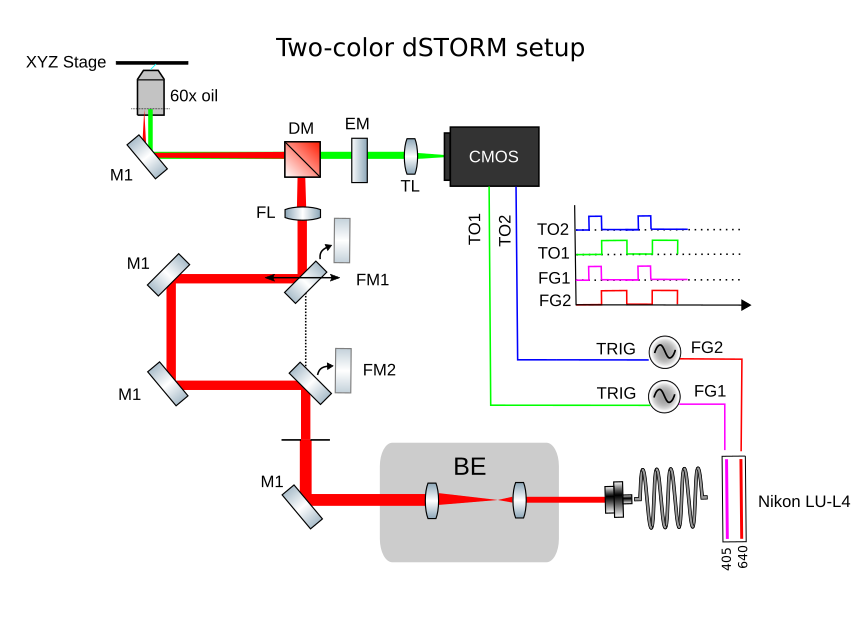
\includegraphics[width=12cm]{dSTORM.png}
\caption{Direct stochastic optical reconstruction microscope}
\end{figure}

\section{Langevin dynamics of a Rouse-like polymer embedded in a transcriptional condensate}

The formation of these transcriptional condensates driven by MED1 and BRD4 alongside decreased entropy of the chromatin scaffold have been previously demonstrated with super-resolution microscopy. Yet, the biophysical descriptions of the interaction between transcriptional condensates with the chromatin fiber and the mechanisms by which they evoke bursty gene expression remain mere speculation. 

Here, we intend to address these outstanding questions by modeling transcriptional condensate formation within a Rouse-like polymer model parameterized by constraints measured in single particle tracking experiments. These models serve to address the stability of transcriptional condensates as a function of their stoichiometry and the relationship between condensate formation and transcriptional bursting by integrating their associated Langevin dynamics with Monte Carlo simulations. 


The general properties of ranscriptional condensates can be investigated using the stochastic simulation algorithm [Gillespie].

 
\bibliographystyle{unsrt}
\bibliography{Dissertation-Transcription.bib}

 
\end{document}